\documentclass{article}

\usepackage{graphicx}

\title{Waves Group Project: Bluetooth}
\author{Lasse Lundberg}

\begin{document}
	\maketitle
	\pagenumbering{gobble}
	\newpage
	
	\pagenumbering{arabic}
	
	\section{Introduction}
		Bluetooth is a wireless communications technology for short-medium range data transfer
	
	\subsection{History of Bluetooth}
		Bluetooth was developed by the Swedish telephone company Ericsson AB in 1990, and it first hit the commercial markets in 1999. It was named after a Danish viking named Harald Blåtand, who's name translates into Bluetooth. 

	\section{The Bluetooth Technology}
		Bluetooth works with radio waves in the frequency range of 2.4 GHz - 2.44835 GHz
	
		\subsection{Frequency Hopping}
			Bluetooth uses a technology known as Adaptive Frequency Hopping, where each package is sent on a different frequency, following a pseudorandom pattern. 
			
			\subsubsection{Pros}
				Substantially higher transfer speeds, as up to 79 different channels can be used at once within the frequency range. It also makes jamming the signal substantially more difficult, since an intruder would not necessarily know the pattern that is being followed. 
			
			\subsubsection{Cons}
				Synchronising the sender and receiver can be difficult but there are techniques for overcoming this, however this is also one of the main contribting factors which slow down initially connecting two Bluetooth devices.
				
	\subsection{Master and Slave Topology}
		Bluetooth follows a master/slave topology where there is a master device broadcasting data to a maximum of seven slave devices. This network of 8 devices is known as a piconet. The master will always default to being the device which initialised the connection, however master and slave roles can be exchanged given that both devices agree upon this. \newline
\begin{figure}
	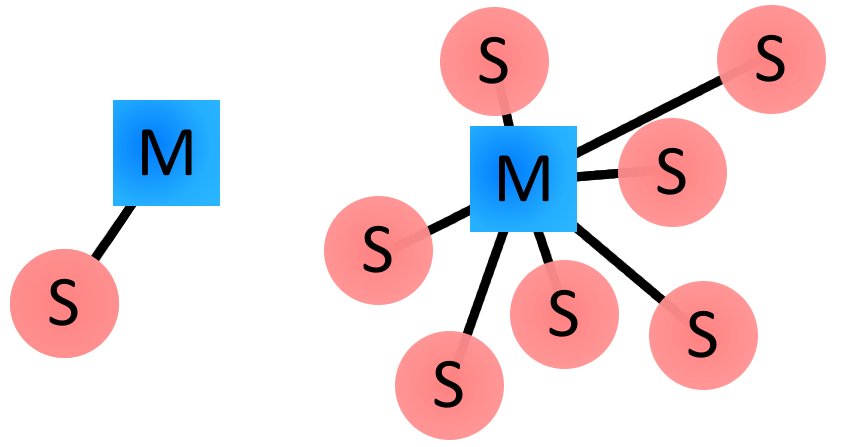
\includegraphics[width=\linewidth]{master_slave_topology.png}
	\caption{Master/Slave topology graph}
\end{figure}	
	
	\section{Short and Snappy}
		- Bluetooth follows a fixed clock rate of $312.5\mu s$ \newline
		- Bluetooth has lots of different implementations for lots of different purposes. Many of these are open source \newline
		- Depending on the type of Bluetooth used, its range varies from under 10 meters up to 100 meters
	
	
\end{document}